\section{Revisión sistemática}

\begin{frame}		
	\begin{block}{Revisión sistemática}
		La revisión de la literatura empezó con un estudio exploratorio seguido de una revisión sistemática. Por lo tanto, fue posible:
		\begin{enumerate}
			\item Encontrar un área de recomendación de vanguardia para flujos de trabajo científicos.
			\item Comprender el problema.
			\item Encuentrar términos específicos del área.
			\item Definir palabras clave
		\end{enumerate}
	\end{block}
\end{frame}

\begin{frame}		
	\begin{block}{Conducir}
		\begin{figure}
			\tiny
			\begin{minipage}[b]{0.46\textwidth}
				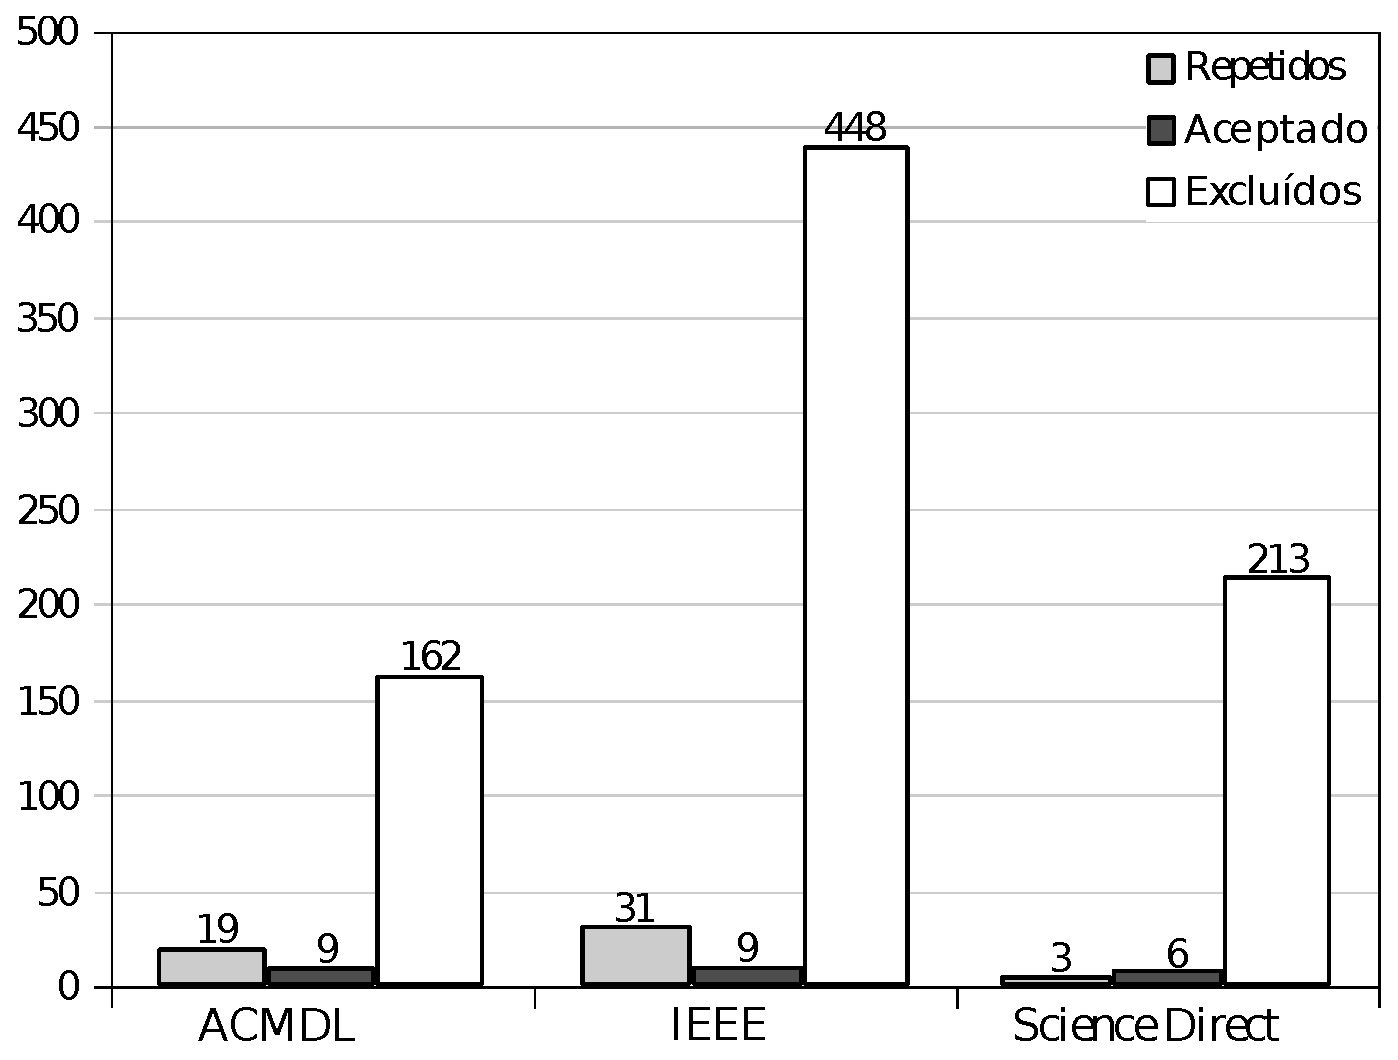
\includegraphics[width=\textwidth]{./secoes/RevisaoDaLiteratura/GraficoQuantidade.eps}
				\caption{Número de artículos por técnica.}
			\end{minipage}
			%\qquad
		     \hspace{0.1cm}
			\begin{minipage}[b]{0.46\textwidth}
				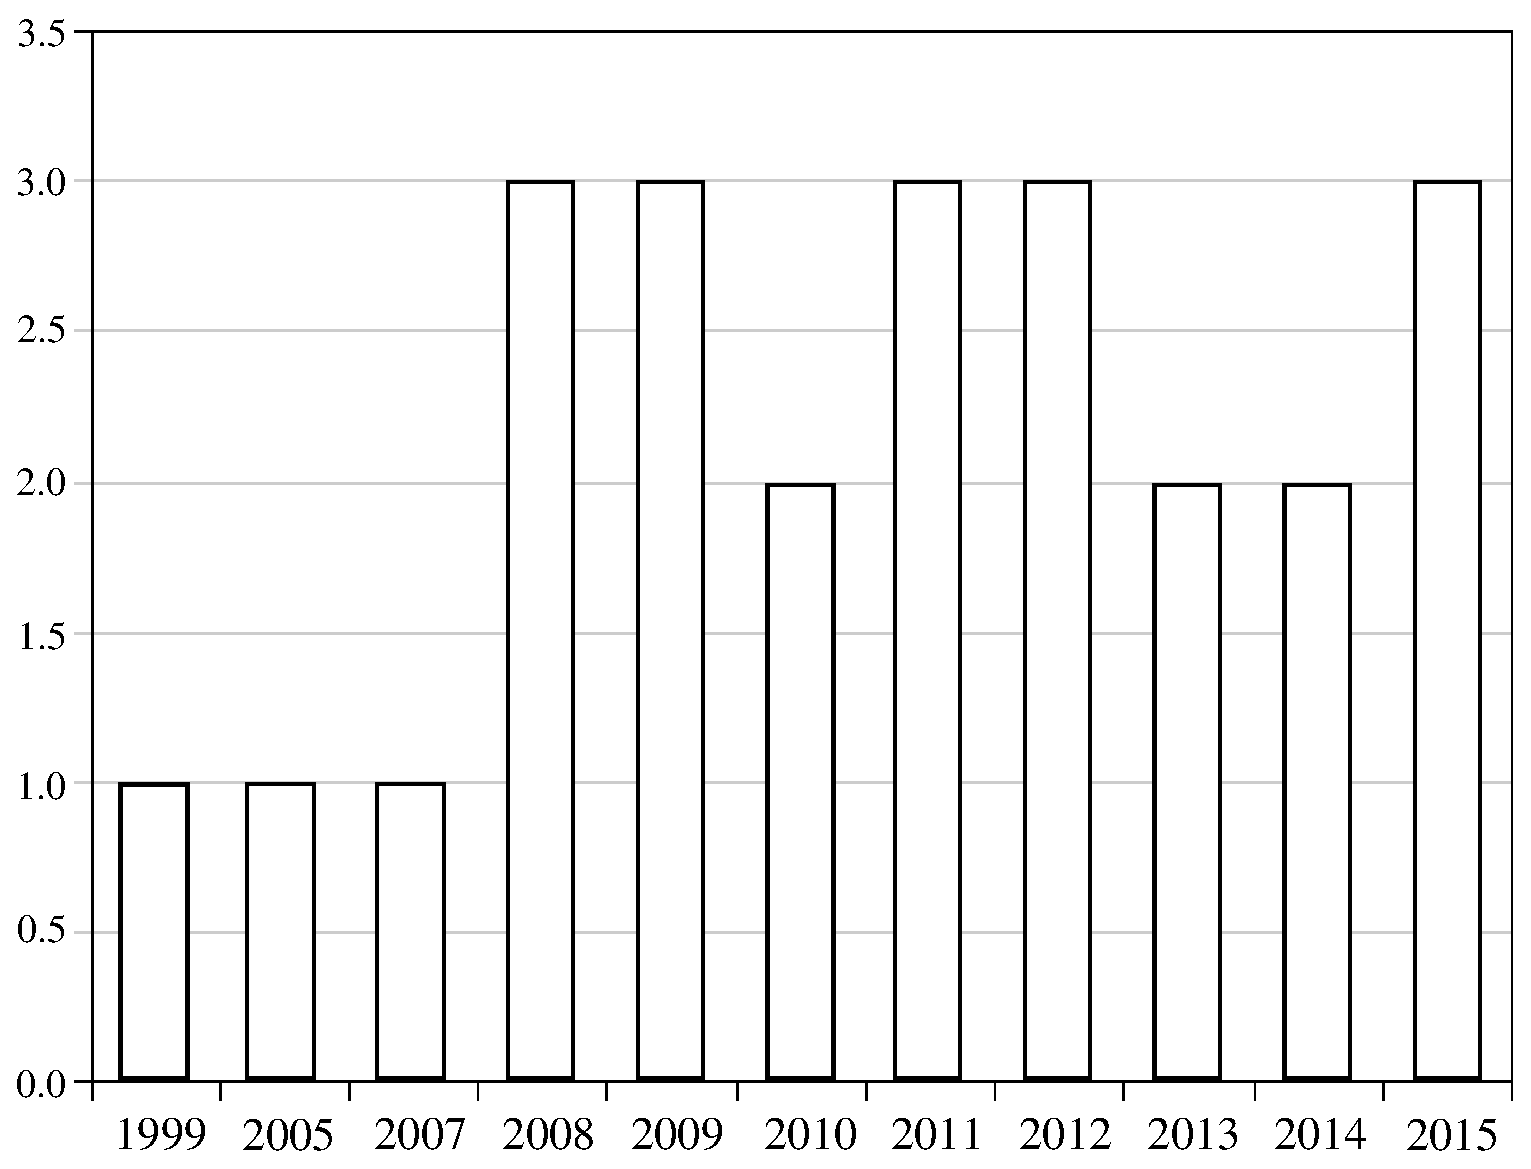
\includegraphics[width=\textwidth]{./secoes/RevisaoDaLiteratura/GraficoQuantidadeAno.eps}
				\caption{Artículos por año de publicación}
			\end{minipage}
		\end{figure}
		
	\end{block}
\end{frame}

\begin{frame}		
	\begin{block}{Ejecución}
		Se observa que la técnica de procedencia es la más utilizada seguida de: i) Frecuencia; ii) entrada y salida; iii) \emph{itemsets}; y iv) ontologías.
		\begin{figure}
			\begin{minipage}[b]{0.5\textwidth}
				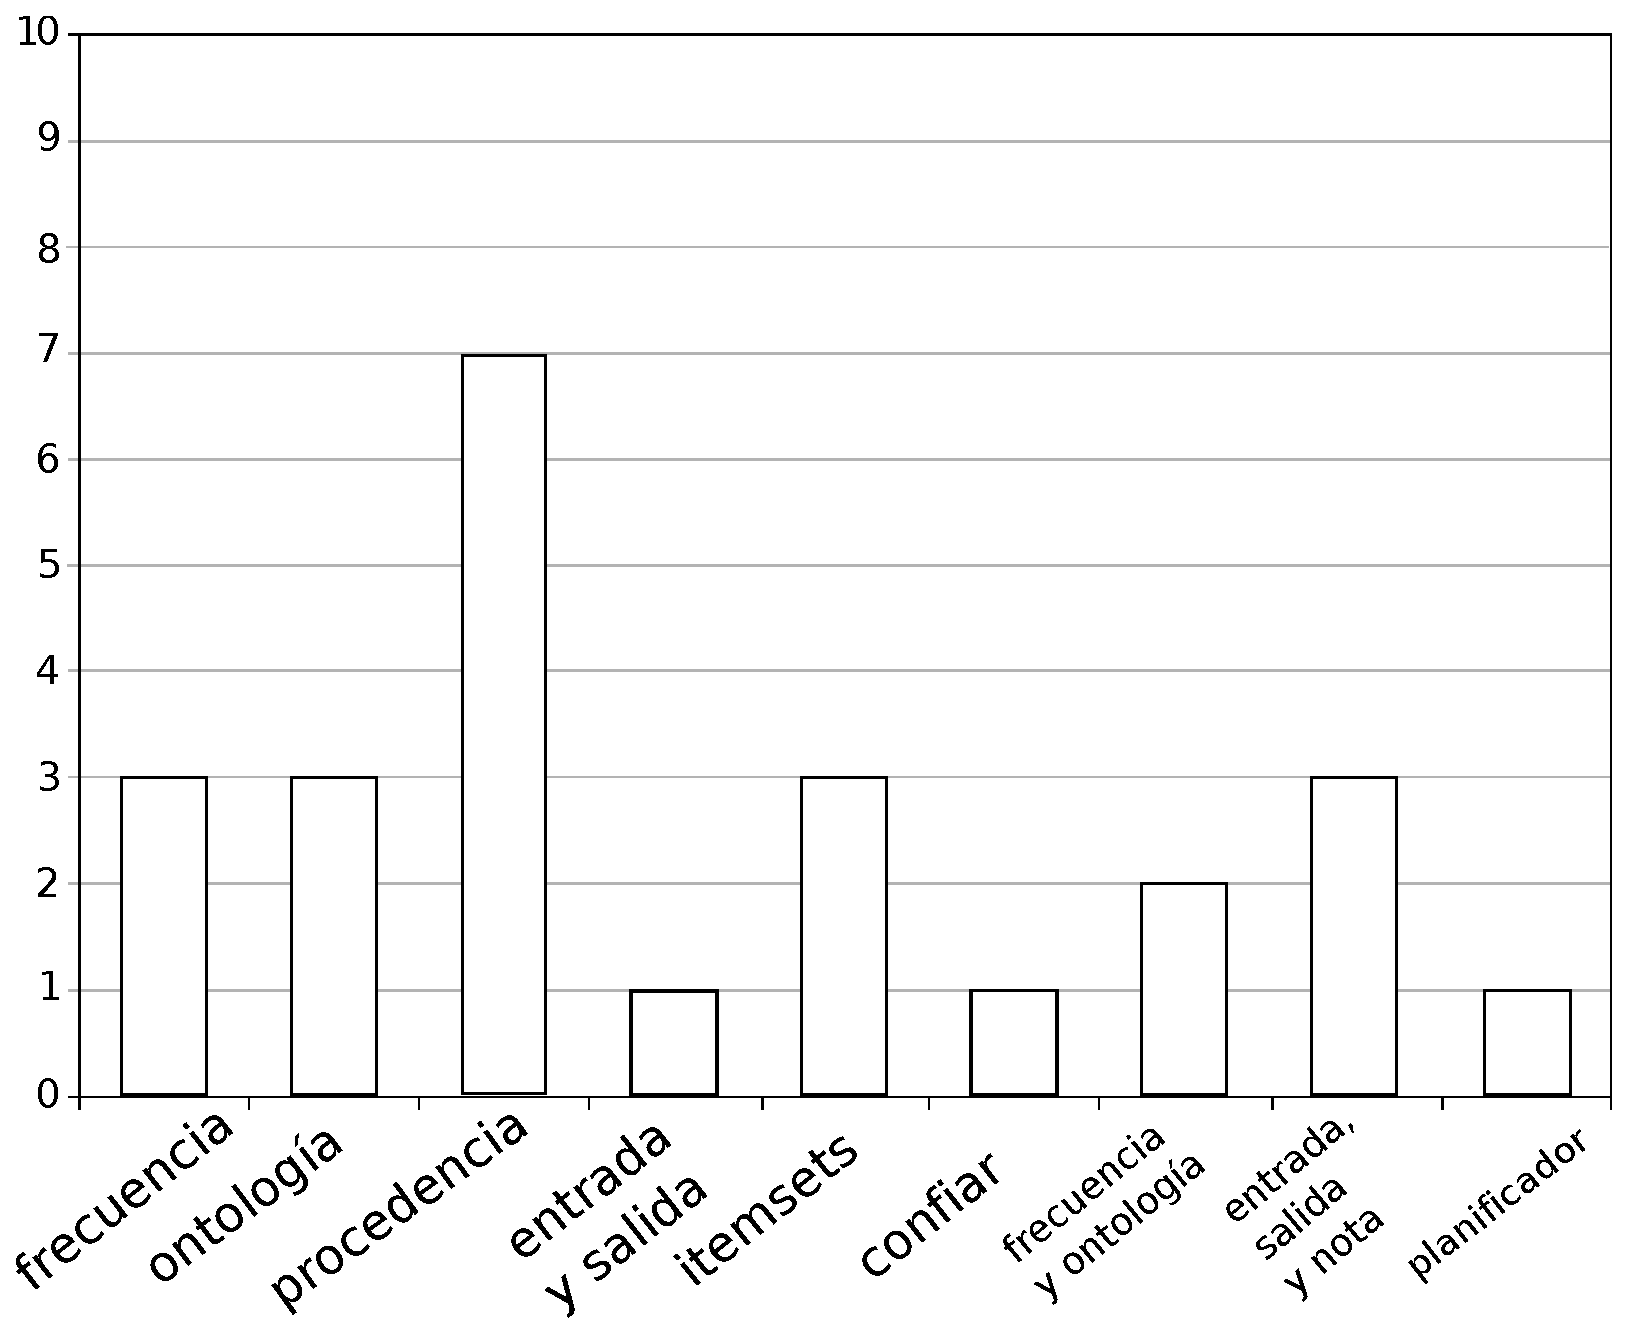
\includegraphics[width=\textwidth]{./secoes/RevisaoDaLiteratura/GraficoQuantidadeTecnica.eps}
%				\caption{Número de artículos por técnica.}
			\end{minipage}
		\end{figure}
		
	\end{block}
\end{frame}

\begin{frame}		
	\begin{block}{Comparación de la técnica propuesta con la literatura relacionada.}
		Las principales ventajas de la técnica propuesta, en relación con las de la literatura relacionada, son considerar las dependencias de entrada y salida, la semántica y la frecuencia de las actividades. 
		
		Además, no se requieren datos de procedencia, redes sociales, recomendacion por confianza entre usuarios o tipo de actividad: i) Shim; ii) Simples; I/O iii) Subflujo de trabajo.
	\end{block}
\end{frame}

